% Created 2016-04-18 Mon 17:08
\documentclass[11pt]{article}
\usepackage[utf8]{inputenc}
\usepackage[T1]{fontenc}
\usepackage{fixltx2e}
\usepackage{graphicx}
\usepackage{grffile}
\usepackage{longtable}
\usepackage{wrapfig}
\usepackage{rotating}
\usepackage[normalem]{ulem}
\usepackage{amsmath}
\usepackage{textcomp}
\usepackage{amssymb}
\usepackage{capt-of}
\usepackage{hyperref}
\author{Nick Anderson}
\date{\today}
\title{Badlock Discovery and Remediation}
\hypersetup{
 pdfauthor={Nick Anderson},
 pdftitle={Badlock Discovery and Remediation},
 pdfkeywords={},
 pdfsubject={},
 pdfcreator={Emacs 24.5.1 (Org mode 8.3.4)},
 pdflang={English}}
\begin{document}

\maketitle
\tableofcontents


\includegraphics[width=.9\linewidth]{../media/badlock.png}


By now you have probably heard about the \href{https://access.redhat.com/security/vulnerabilities/badlock}{Badlock vulnerability} (\href{https://cve.mitre.org/cgi-bin/cvename.cgi?name=CVE-2016-2118}{CVE-2016-2118})
in DCE/RPC-based SAMR and LSA protocols used in the Microsoft Windows Active
Directory infrastructure as well as other \href{https://access.redhat.com/articles/2243351}{critical security flows in Samba}.

With CFEngine Enterprise you can simply tag any variable or class and Mission
Portals Inventory reporting interface will be automatically extended with the
new attributes. This makes it easy to identify vulnerable hosts.

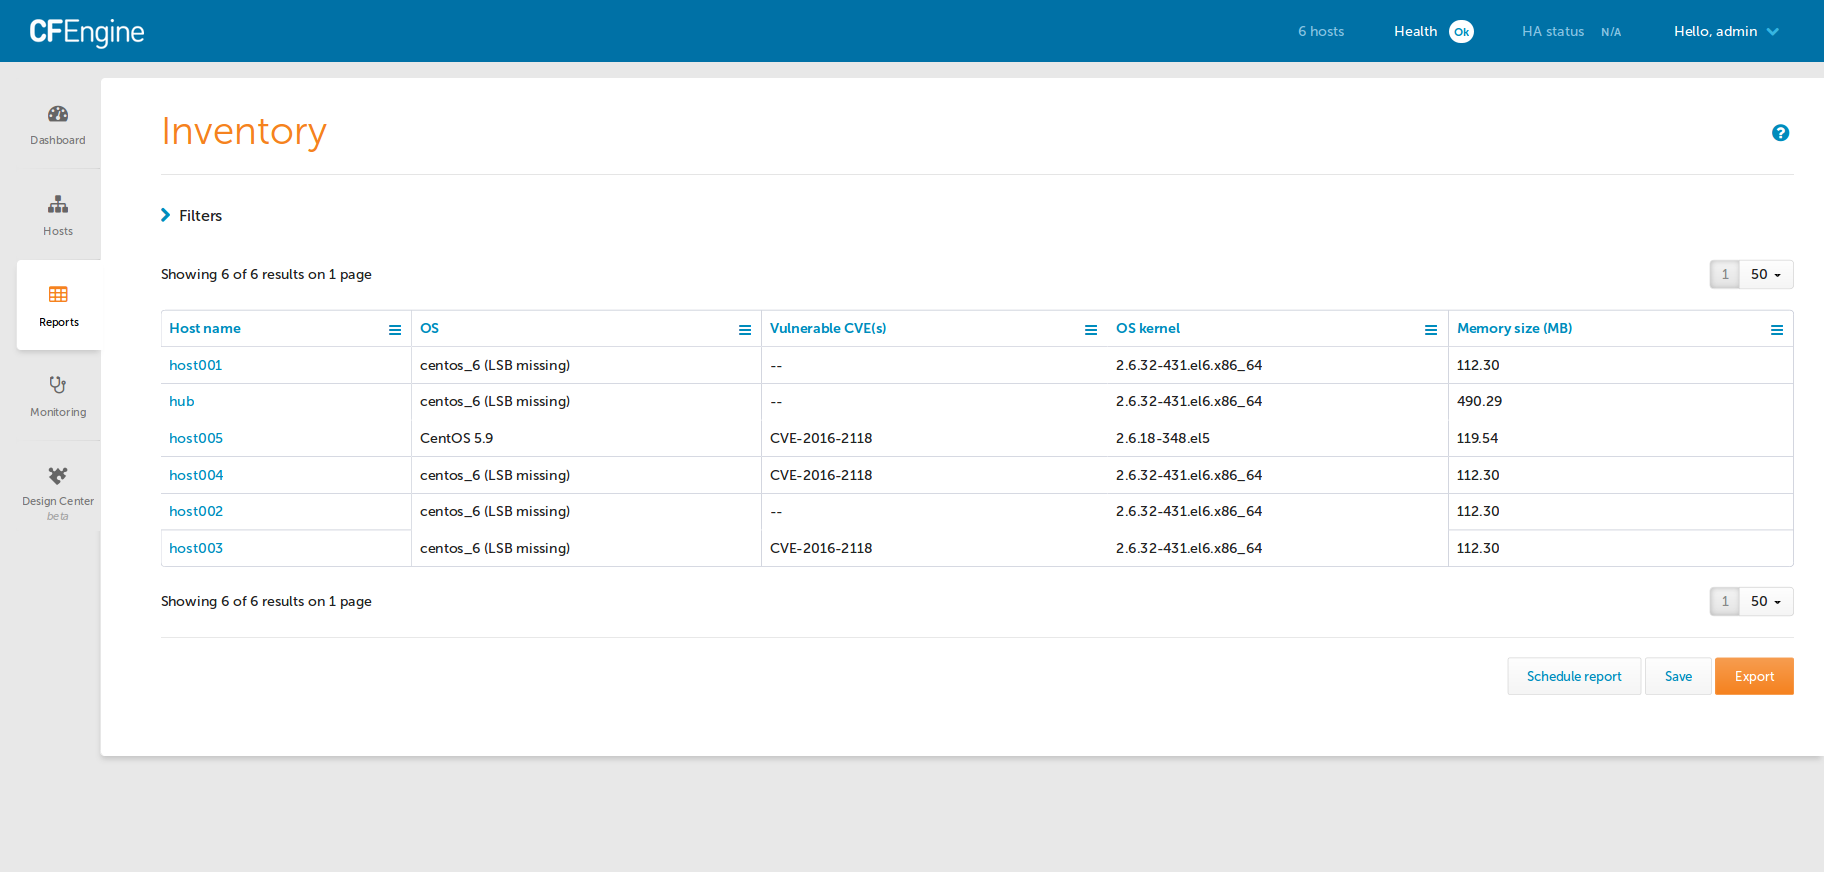
\includegraphics[width=.9\linewidth]{../media/inventory_report_vulnerable_cves.png}

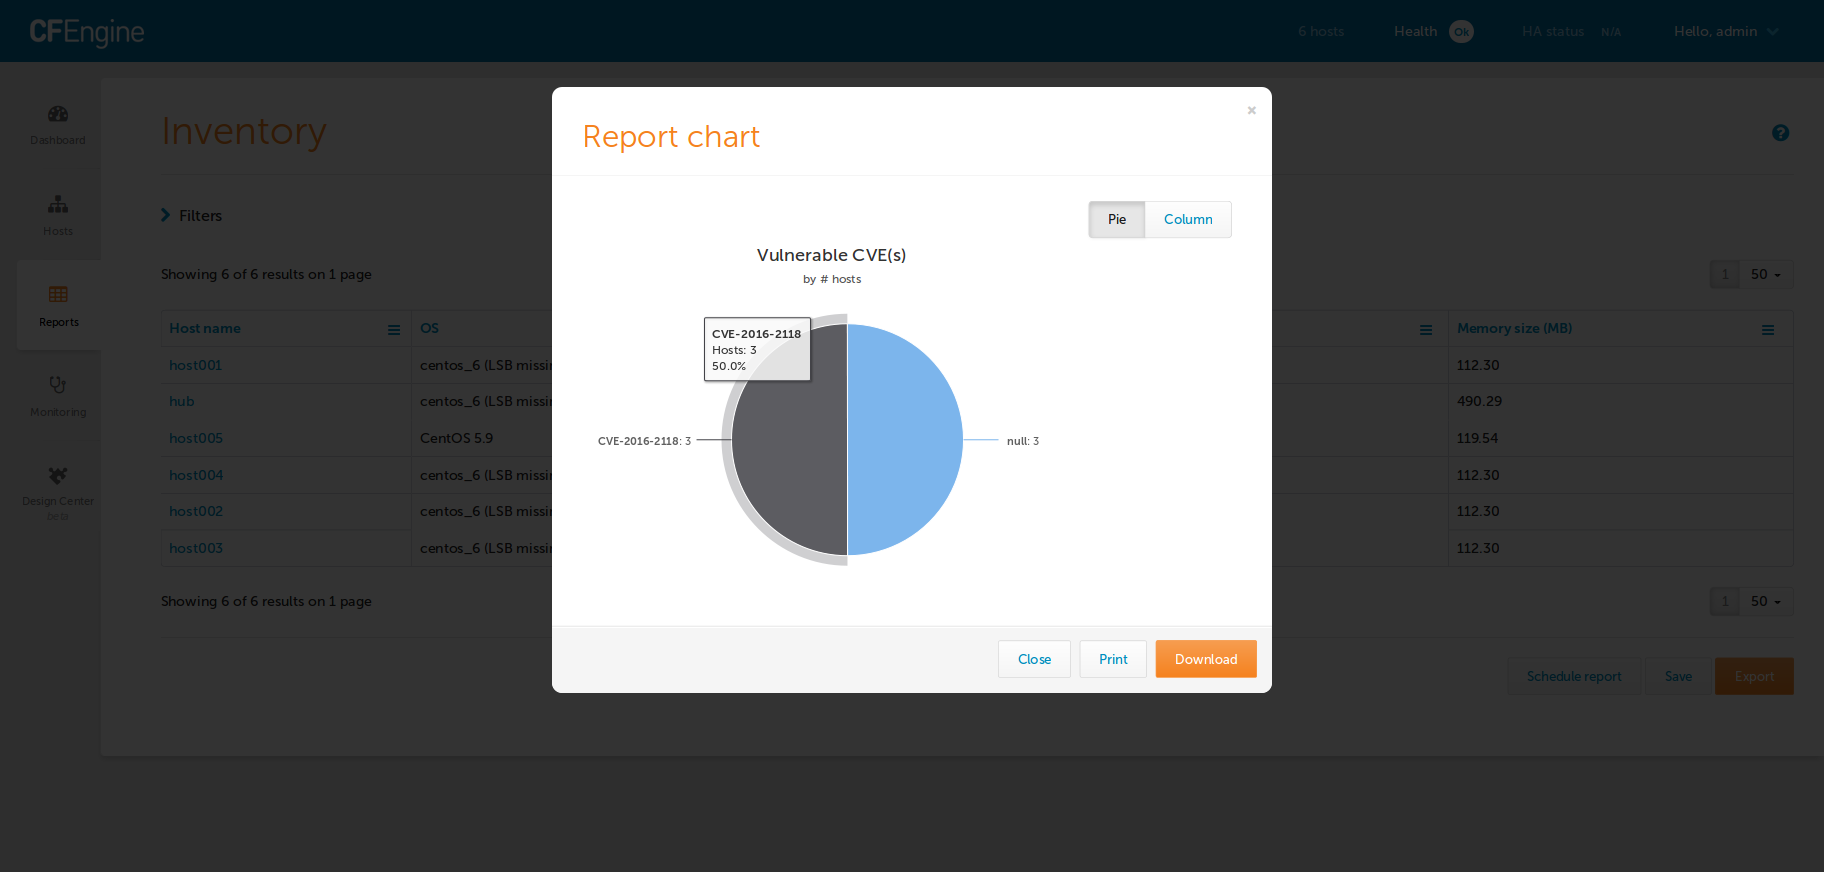
\includegraphics[width=.9\linewidth]{../media/inventory_report_vulnerable_cves_chart.png}

Dashboard alerts can be created to alert on vulnerable hosts on specific subsets
of infrastructure.

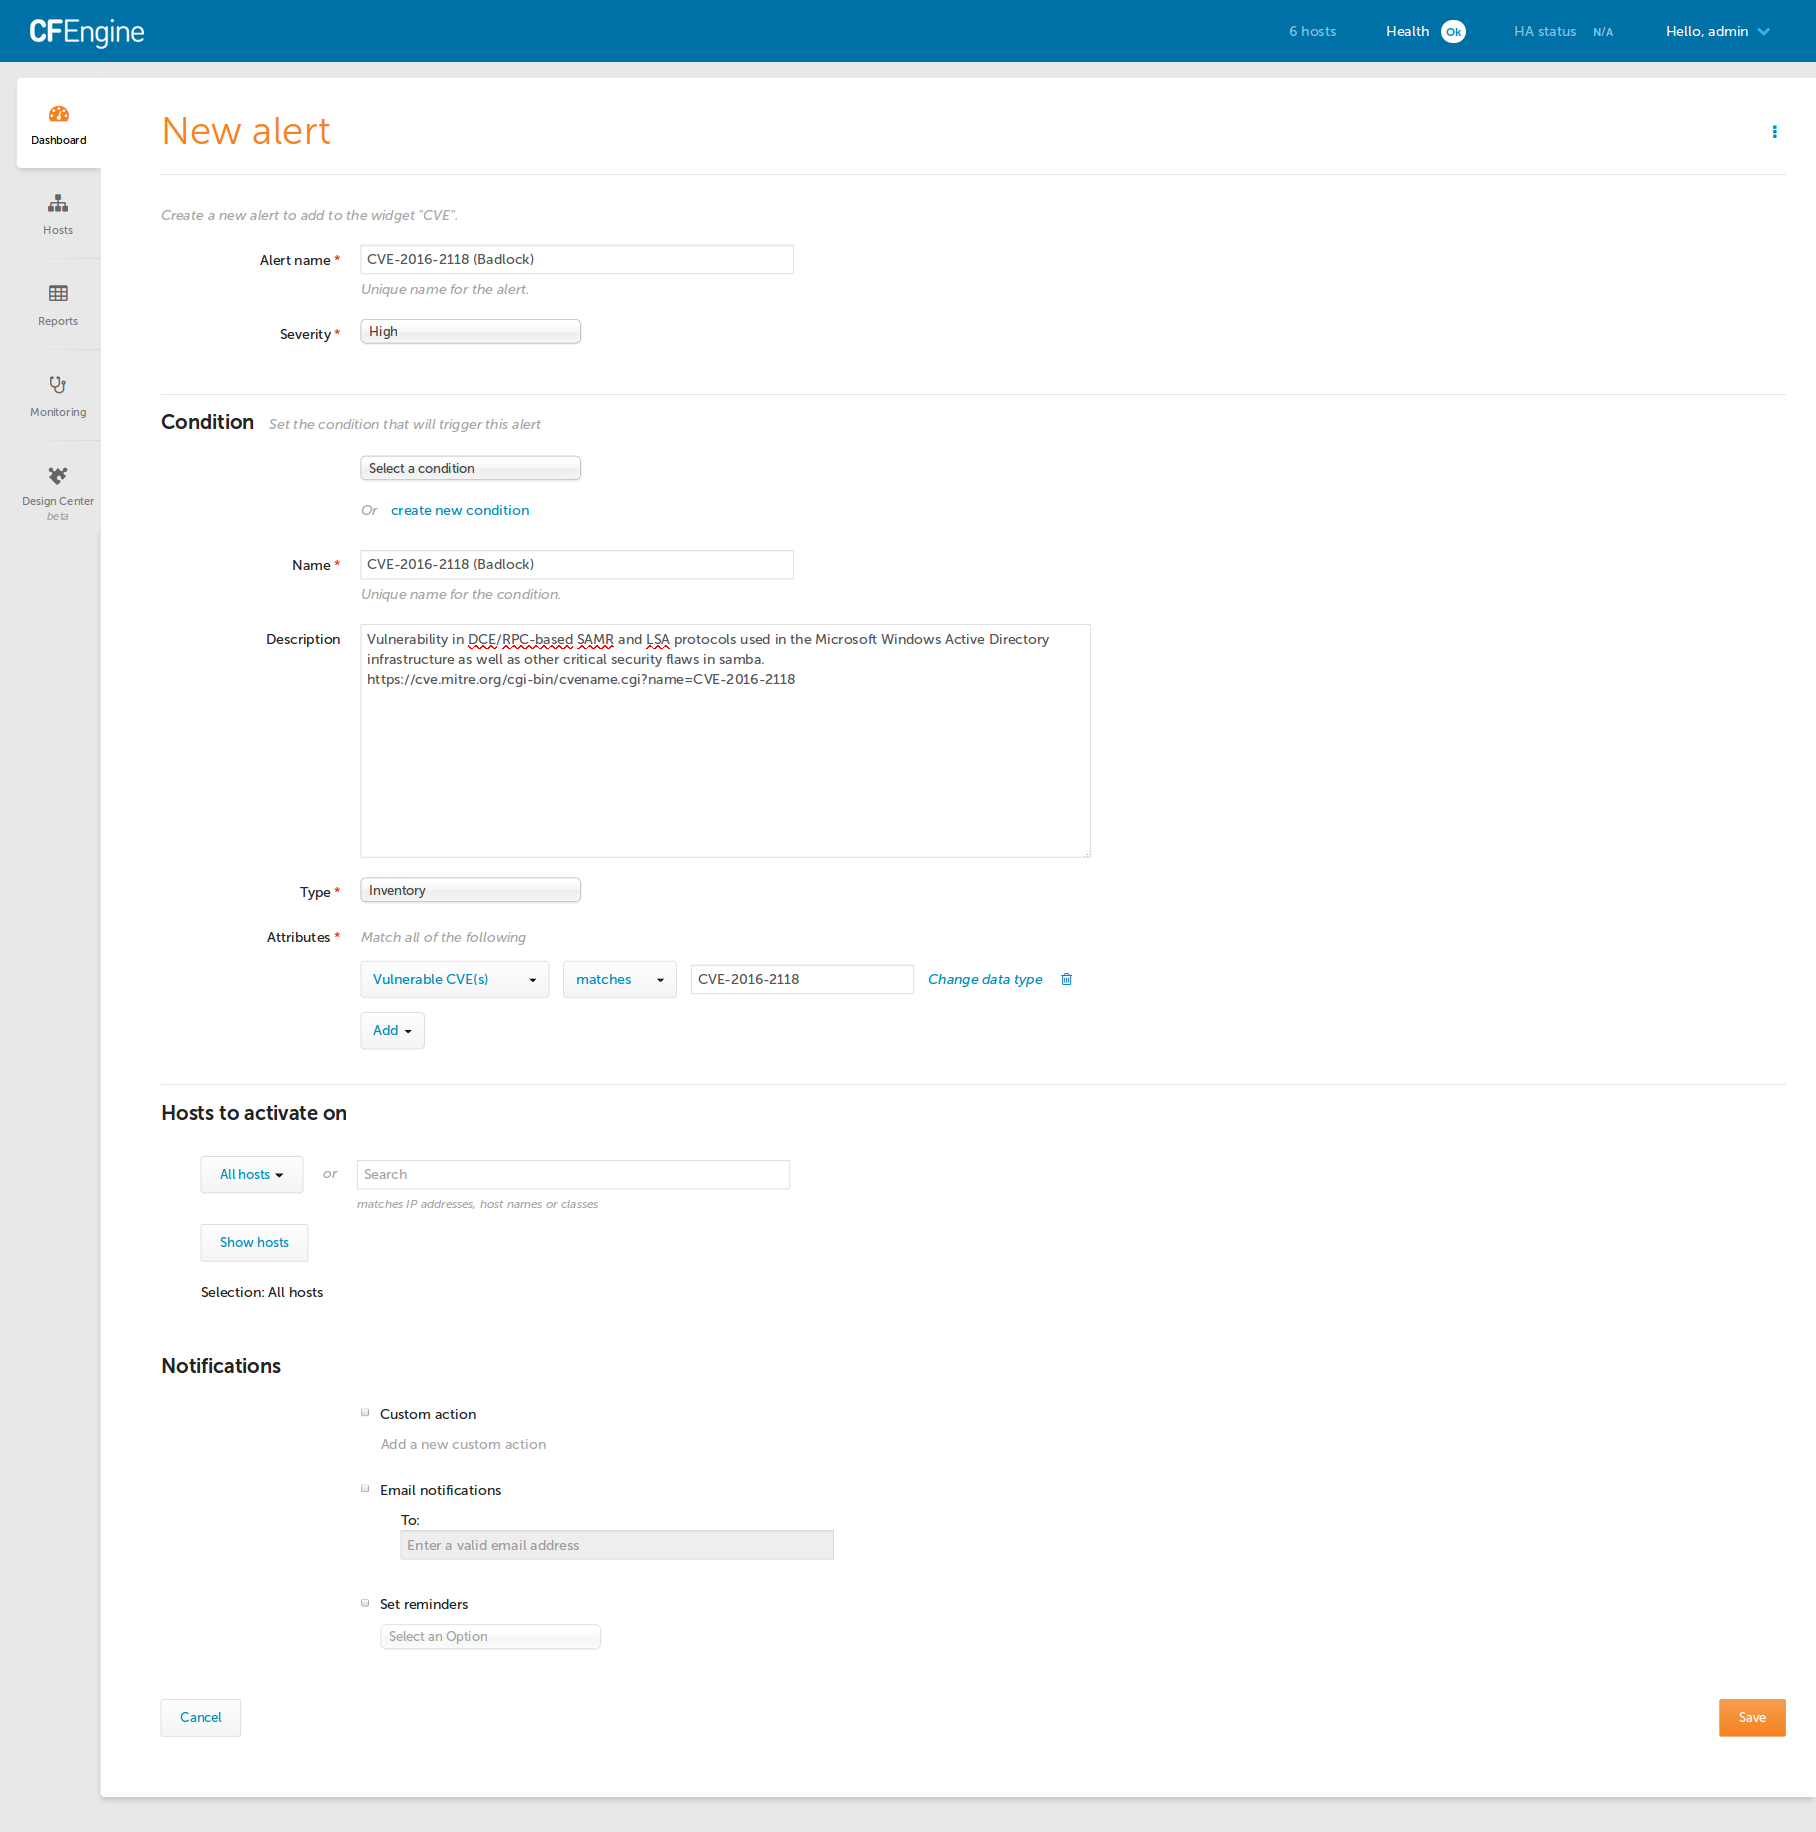
\includegraphics[width=.9\linewidth]{../media/define_alert.png}

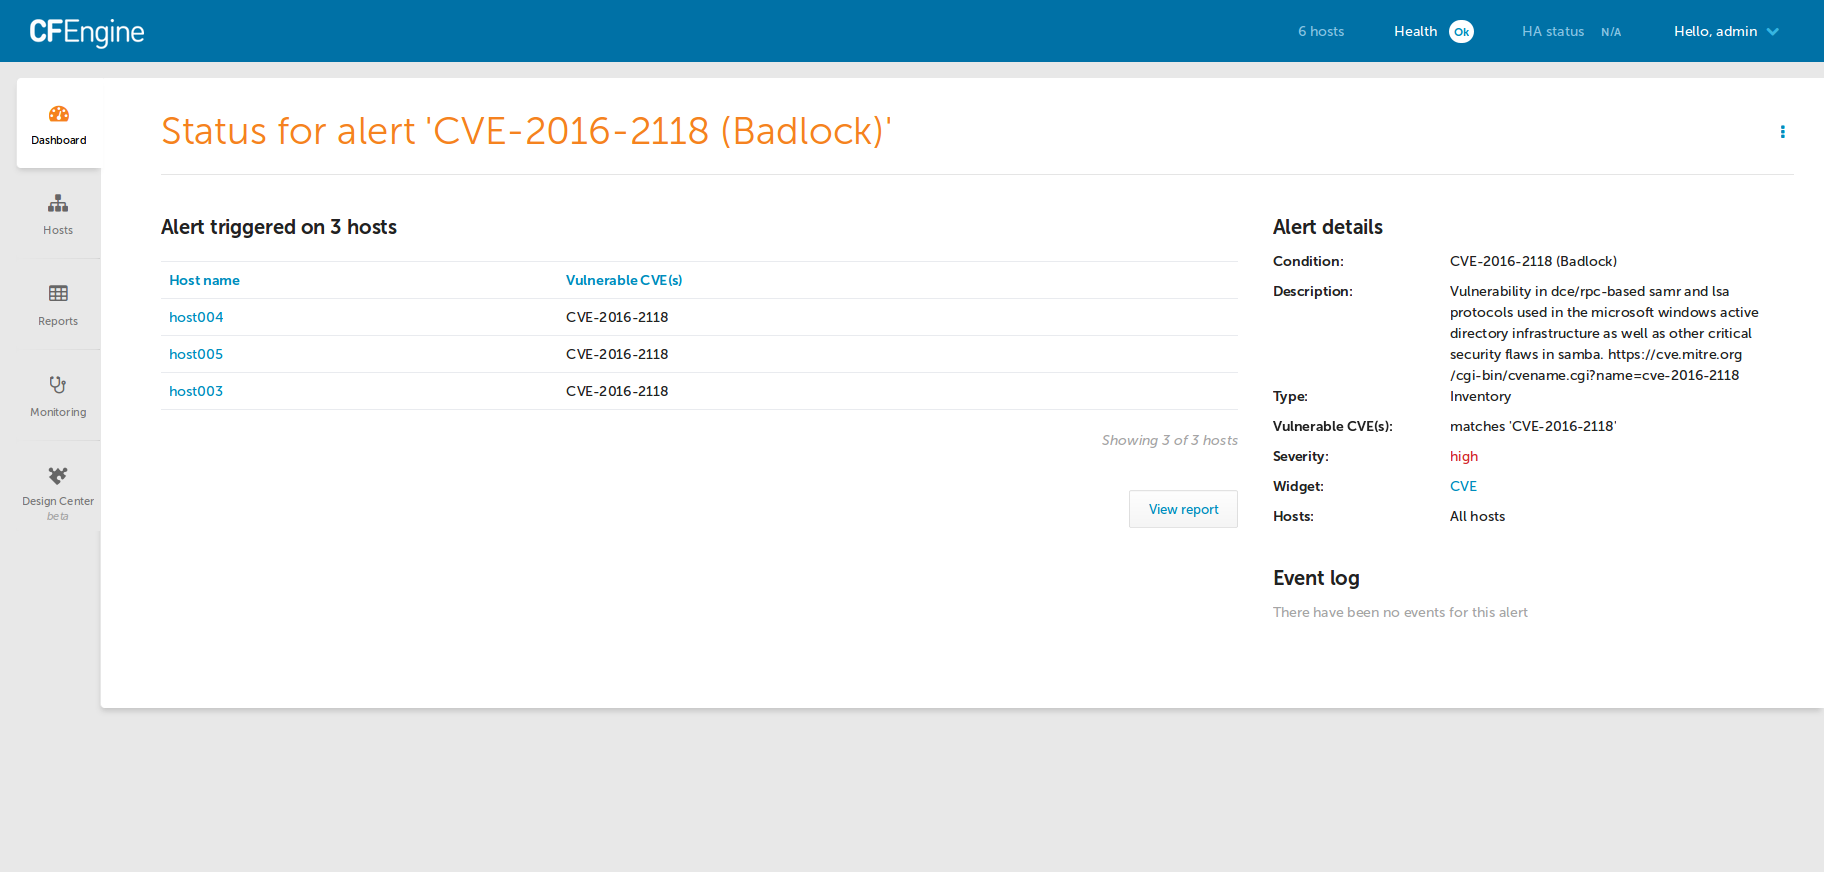
\includegraphics[width=.9\linewidth]{../media/alert_status_vulnerable_hosts.png}

Dashboard alerts can be \href{https://cfengine.com/learn/integrate-with-other-tools/}{integrated with other systems}. For example you could
\href{https://cfengine.com/learn/ticketing-system-integration-jira/}{automatically open an issue in Jira} when vulnerable hosts are found.

If you would like to use CFEngine to detect, repair and report on Badlock in
your infrastructure, we have prepared some policies you can use.
\begin{itemize}
\item Example \href{https://github.com/nickanderson/cfengine-CVE-2016-2118}{Badlock reporting and remediation policy}
\item Example Implementation Tutorial
\end{itemize}

We want to have a good understanding of which systems are vulnerable before we
start patching services. There are several ways to accomplish this, for this
example we chose to enumerate all of the package versions that are known to be
vulnerable. The information about which package versions are vulnerable can be
obtained from your operating system vendor (and sometimes directly from your
package manager).

I have the list of vulnerable versions of samba in a json data file named for
the platform as detected by CFEngine as \texttt{\$(sys.flavor)}. This is the contents of
the CentOS 6 vulnerable packages for samba (\texttt{data/centos\_6.json}).

\begin{verbatim}
[
    "3.5.4-68.el6",
    "3.5.4-68.el6_0.1",
    "3.5.4-68.el6_0.2",
    "3.5.6-86.el6",
    "3.5.6-86.el6_1.4",
    "3.5.10-114.el6",
    "3.5.4-68.el6_0.3",
    "3.5.10-115.el6_2",
    "3.5.6-86.el6_1.5",
    "3.5.10-116.el6_2",
    "3.5.10-125.el6",
    "3.6.9-151.el6",
    "3.6.9-151.el6_4.1",
    "3.6.9-160.3.el6rhs",
    "3.6.9-164.el6",
    "3.6.9-160.7.el6rhs",
    "3.6.9-167.el6_5",
    "3.6.9-167.5.1.el6rhs",
    "3.6.9-167.10.el6rhs",
    "3.6.9-168.el6_5",
    "3.6.23-12.el6",
    "3.6.9-169.el6_5",
    "3.6.9-169.1.el6rhs",
    "3.6.509-169.1.el6rhs",
    "3.6.509-169.4.el6rhs",
    "3.6.9-167.10.1.el6rhs",
    "3.6.23-14.el6_6",
    "3.6.9-151.el6_4.3",
    "3.6.9-171.el6_5",
    "3.5.10-119.el6_2",
    "3.6.509-169.6.el6rhs",
    "3.6.9-167.10.3.el6rhs",
    "4.1.17-4.el6rhs",
    "3.6.23-20.el6",
    "4.1.17-13.el6rhs",
    "4.1.17-14.el6rhs",
    "3.6.23-21.el6_7",
    "3.6.23-24.el6_7",
    "4.1.17-16.el6rhs",
    "4.2.4-13.el6rhs",
    "4.2.4-15.el6rhs",
    "3.6.23-25.el6_7",
    "3.6.23-9.el6"
]
\end{verbatim}

The bundle \texttt{inventory\_CVE\_2016\_2118} uses this data file to detect if a
vulnerable version of samba is installed. If a vulnerable version is found the
class \texttt{CVE\_2016\_2118} is defined, a report indicating the host is vulnerable is
emitted.

\begin{verbatim}
bundle agent inventory_CVE_2016_2118
{
  meta:
    "description"
     string => "Detect and Report on badlock vulnerability.";

    "tags" slist => { "autorun" };

  vars:
    "CVE" string => "CVE-2016-2118";

    "data"
      data => readdata("$(this.promise_dirname)/data/$(sys.flavor).json", "auto"),
      unless => isvariable(data),
      comment => "We have defined the vulnerable package versions for each
      platform we care about in this external data file, we need
      this information so that we can identify if the system has a
                  vulnerable version installed.";

    # We need to extract a list of the versions from the loaded data so that we
    # can compare the list with the installed version of samba (if installed).
    "vulnerable_versions"
      slist => getvalues(data),
      unless => isvariable(vulnerable_versions);

    "packages"
      data => packagesmatching("samba", ".*", ".*", ".*");

  classes:

    # Note: Classes are automatically canonified when defined, but when tested
    # they must be explicitly canonified

    "$(CVE)" -> { "$(CVE)" }
      expression => reglist( @(vulnerable_versions), "$(packages[0][version])" ),
      scope => "namespace",
      comment => "We are vulnerable if the installed version of samba matches a
      vulnerable version as defined in the external data file. We
      define a class for the CVE so that it can be used for making
                  decisions in other parts of the policy";

  vars:

    # CFEngine Enterprise users can tag variables (or classes for that matter)
    # and augment Mission Portals Inventory reporting interface.

    enterprise_edition::

      "vulnerability" -> { "Mission Portal" }
        string => "$(CVE)",
        meta => { "inventory", "attribute_name=Vulnerable CVE(s)" },
        if => canonify( $(CVE) );

  methods:

    "Refresh Installed Software Cache"
      usebundle => refresh_software_package_cache( $(this.bundle) ),
      if => canonify( $(CVE) );

  vars:

    "DEBUG|DEBUG_$(this.bundle)"::

      "updates"
        data => packageupdatesmatching("samba", ".*", ".*", ".*");
      "u" slist => getindices(updates);

      "rpm_q_version"
        string => execresult("/bin/rpm -q samba", "noshell"),
        unless => isvariable( "rpm_q_version" );

    "yum_check_update"
        string => execresult("$(paths.yum) check-update samba", "noshell"),
        unless => isvariable( "yum_check_update" );

  reports:
      "Detected Vulnerability: $(CVE)$(const.n)"
        if => canonify( $(CVE) );

    "DEBUG|DEBUG_$(this.bundle)"::
      "$(const.t)Installed Version:
$(const.t)$(const.t)packagesmatching(): $(packages[0][version])
$(const.t)$(const.t)          `rpm -q`: $(rpm_q_version)$(const.n)";

      "$(const.t)Updates Available:
$(const.t)$(const.t)packageupdatesmatching(samba): $(updates[$(u)][version])
$(const.t)$(const.t)yum check-update samba$(const.n)$(yum_check_update)$(const.n)";
}
\end{verbatim}

If your running CFEngine Enterprise, Mission Portal's Inventory Reporting
interface will be populated with information about the vulnerabilities detected
for each host.

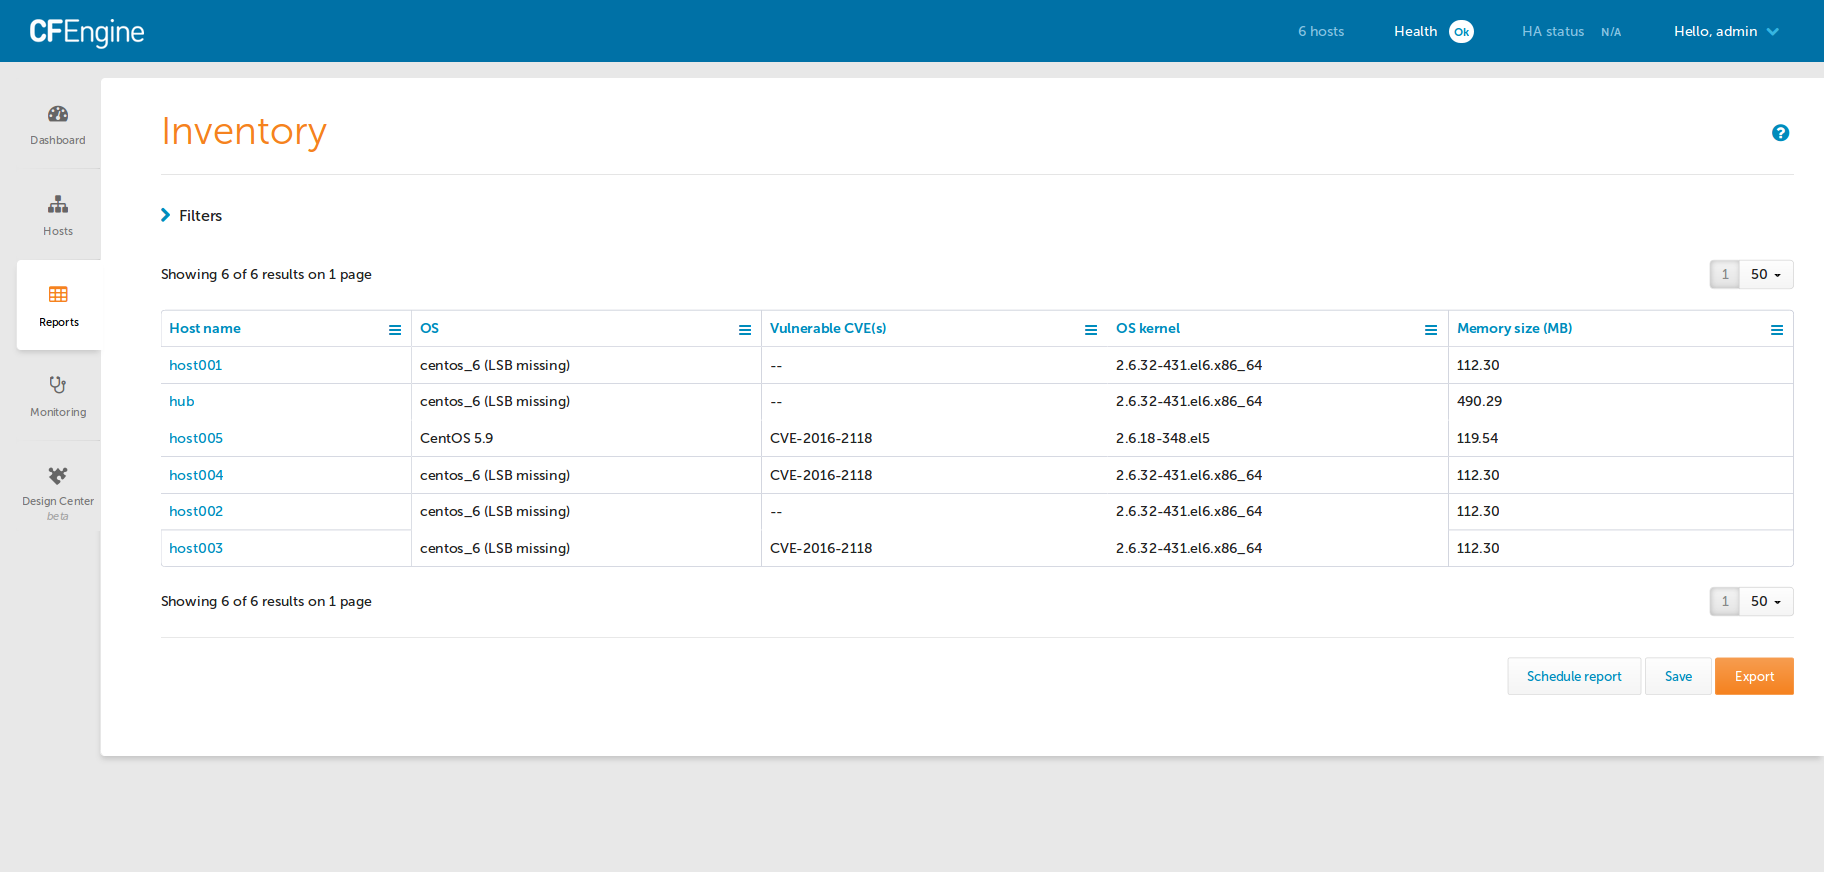
\includegraphics[width=.9\linewidth]{../media/inventory_report_vulnerable_cves.png}

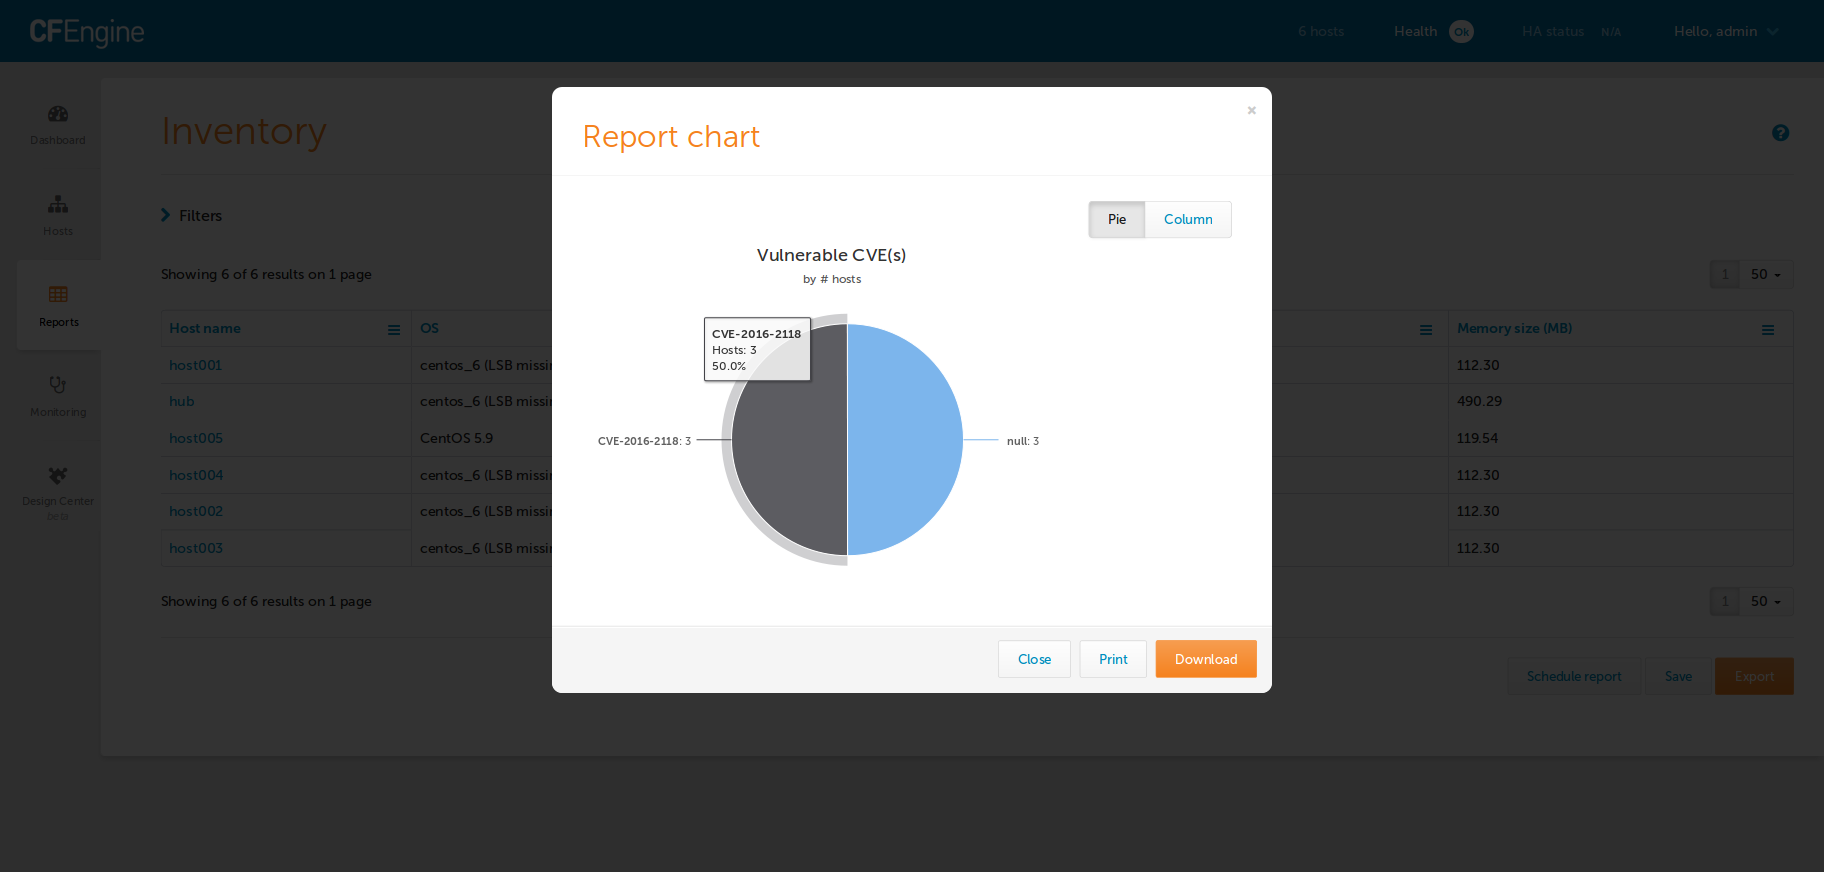
\includegraphics[width=.9\linewidth]{../media/inventory_report_vulnerable_cves_chart.png}

Now that we have the inventory, we can create a dashboard widget and alert to
make vulnerable hosts more vi sable or even \href{https://cfengine.com/learn/ticketing-system-integration-jira/}{integrate it with a custom action}.

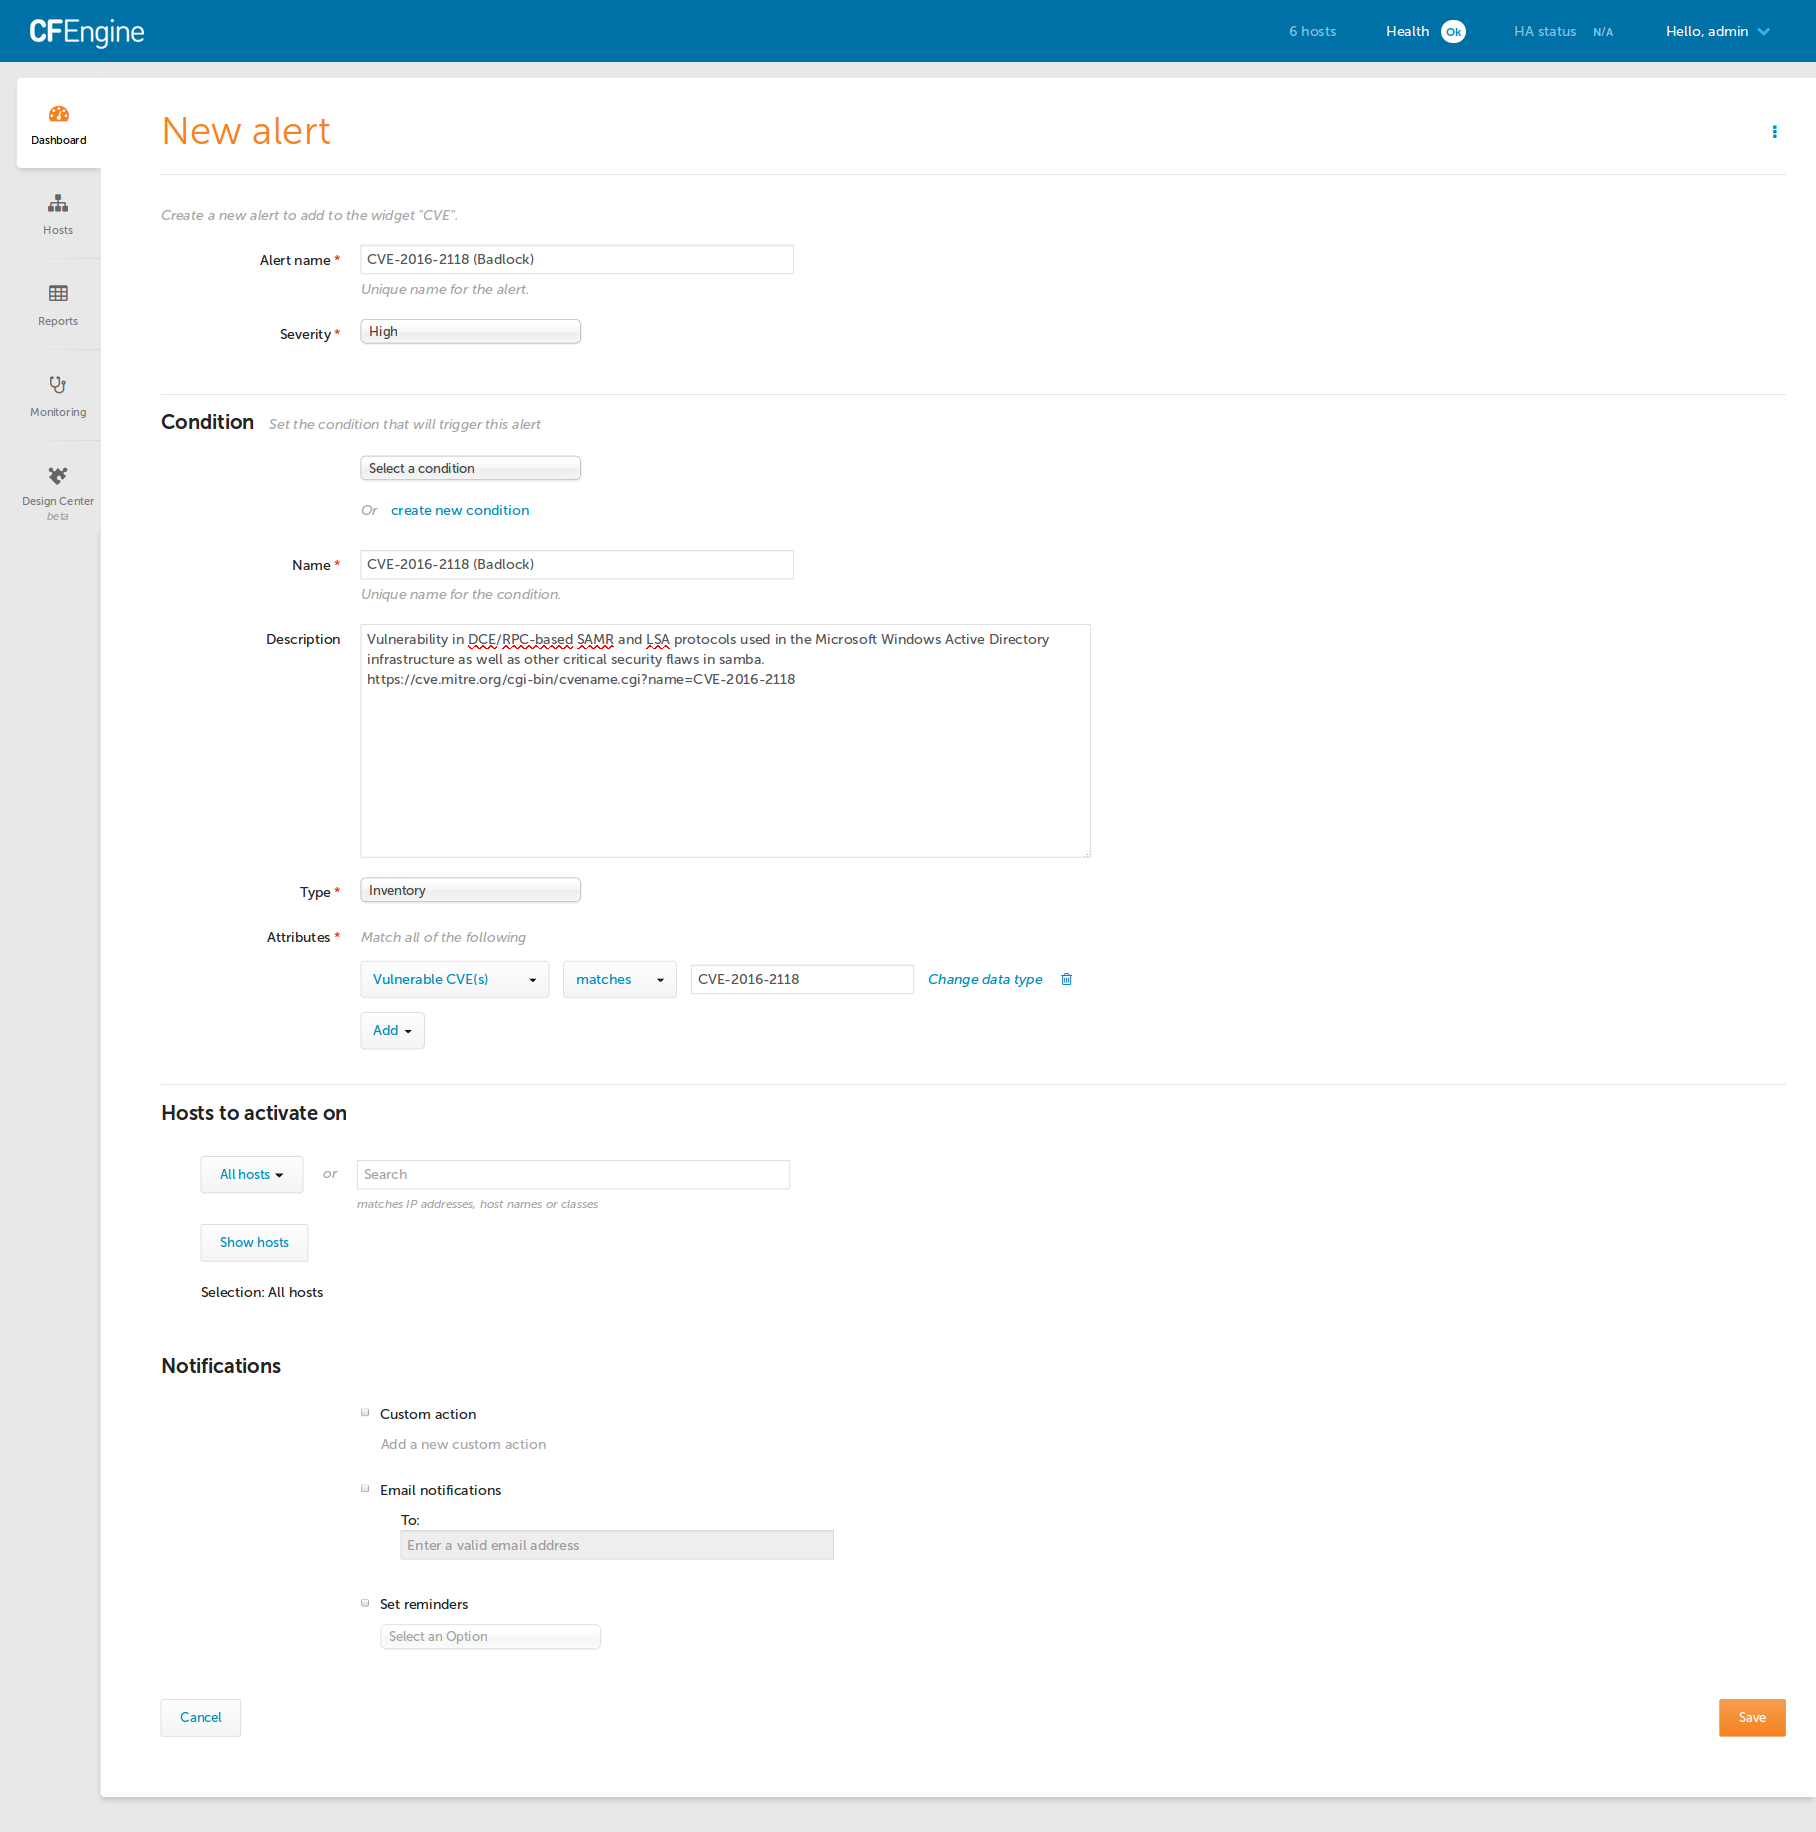
\includegraphics[width=.9\linewidth]{../media/define_alert.png}

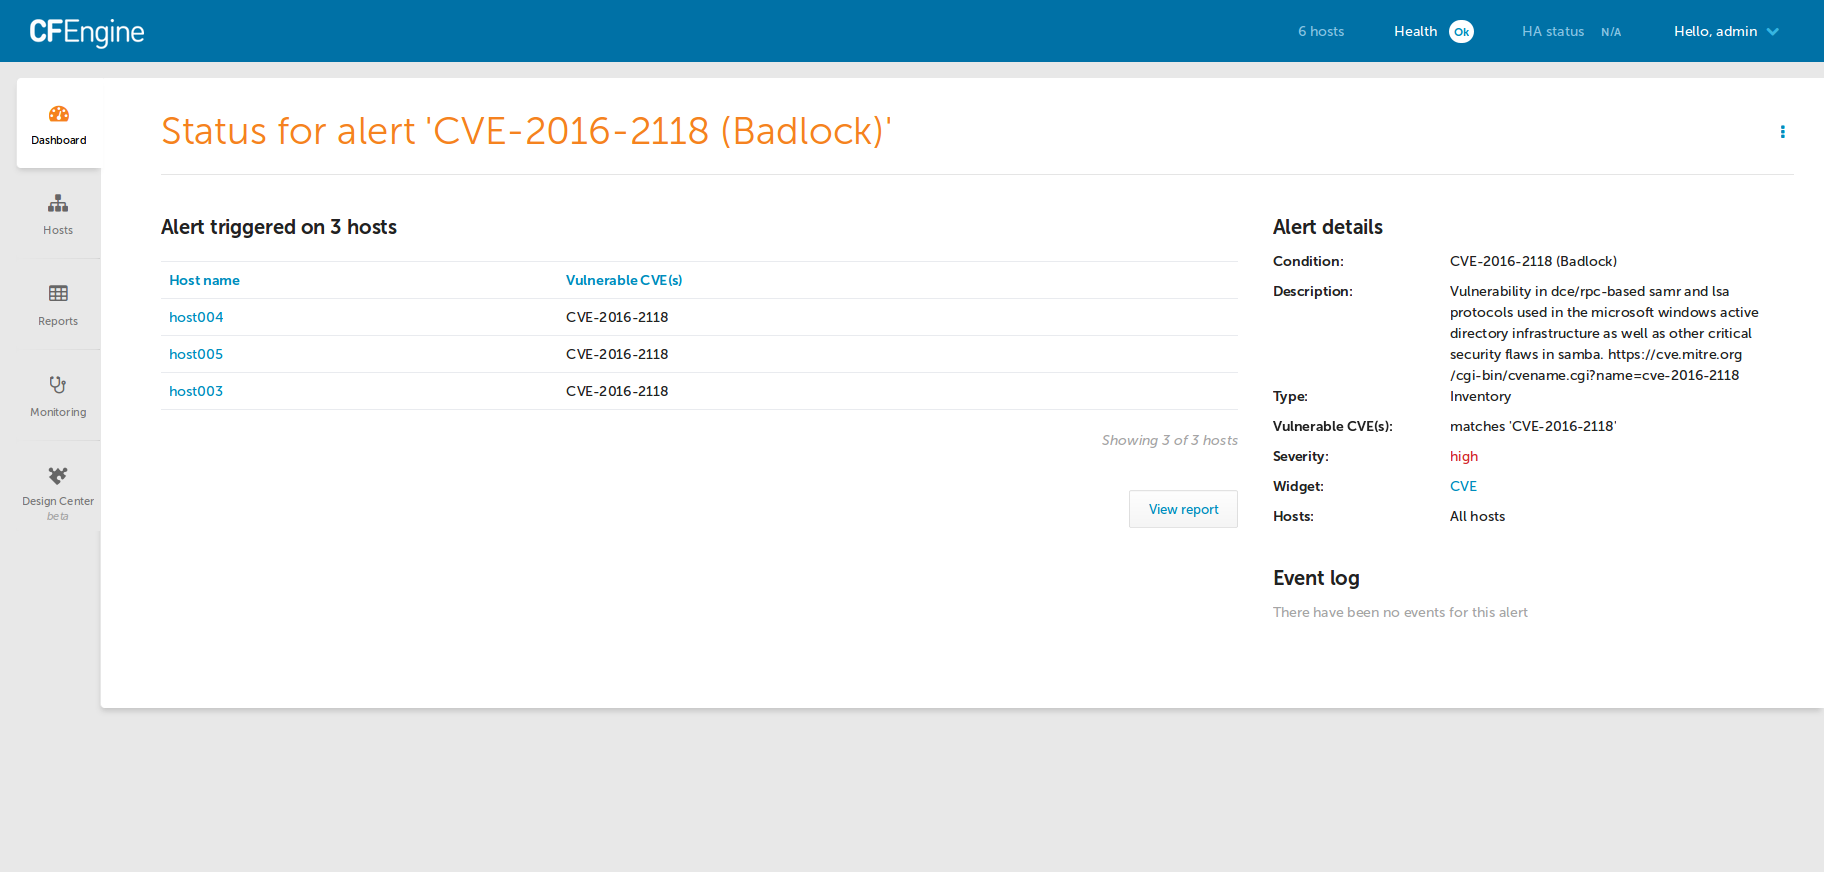
\includegraphics[width=.9\linewidth]{../media/alert_status_vulnerable_hosts.png}

Now with a good understanding of which hosts are vulnerable, we can proceed on
to remediation.

The bundle \texttt{remediate\_CVE\_2016\_2118} ensures samba is the latest version
available if the class \texttt{CVE\_2016\_2118} is detected.

\begin{verbatim}
bundle agent remediate_CVE_2016_2118
{
  meta:
    "description"
      string => "Upgrade samba if we are vulnerable to badlock";

    remediate_CVE_2016_2118::

      "tags" slist => { "autorun" };

  packages:

    centos::

      "samba"
        policy => "present",
        version => "latest",
        package_module => yum,
        classes => results("bundle", "samba_latest"),
        action => immediate,
        if => canonify( $(inventory_CVE_2016_2118.CVE) ),
        comment => "We want to update samba to the latest version available if we
                    are vulnerable.";

  methods:

    "Refresh Installed Software Cache"
      usebundle => refresh_software_package_cache( $(this.bundle) ),
      if => canonify( $(inventory_CVE_2016_2118.CVE) );
}
\end{verbatim}
\end{document}
